\documentclass[a4paper, 11pt]{article}
\usepackage{geometry}
\usepackage{graphicx}
\usepackage{a4wide}
\usepackage{ulem}
\usepackage{amsthm}
\usepackage{amsmath}
\usepackage{amsfonts}
\usepackage{amssymb}
\usepackage[T1]{fontenc}
\usepackage{ngerman}
\usepackage{graphicx}
\usepackage{epic}
\usepackage{enumerate}
\usepackage{tabu}
\usepackage [latin1]{inputenc}
\geometry{a4paper,left=15mm,right=25mm,top=10mm,bottom=15mm}
%\renewcommand{\baselinestretch}{1.5}
\newcommand{\ol}{\overline}
\newcommand{\makeline}{\hrule\vspace{5pt}}
\newcommand{\ip}[2]{\left< #1, #2 \right>}

\title{6. �bungsblatt zu Software Qualit�t}
\author{Michel Meyer, Manuel Schwarz}

\begin{document}
  \maketitle

  \section*{Aufgabe 6.1}
  \subsection*{(a)}
  %\begin{figure}
		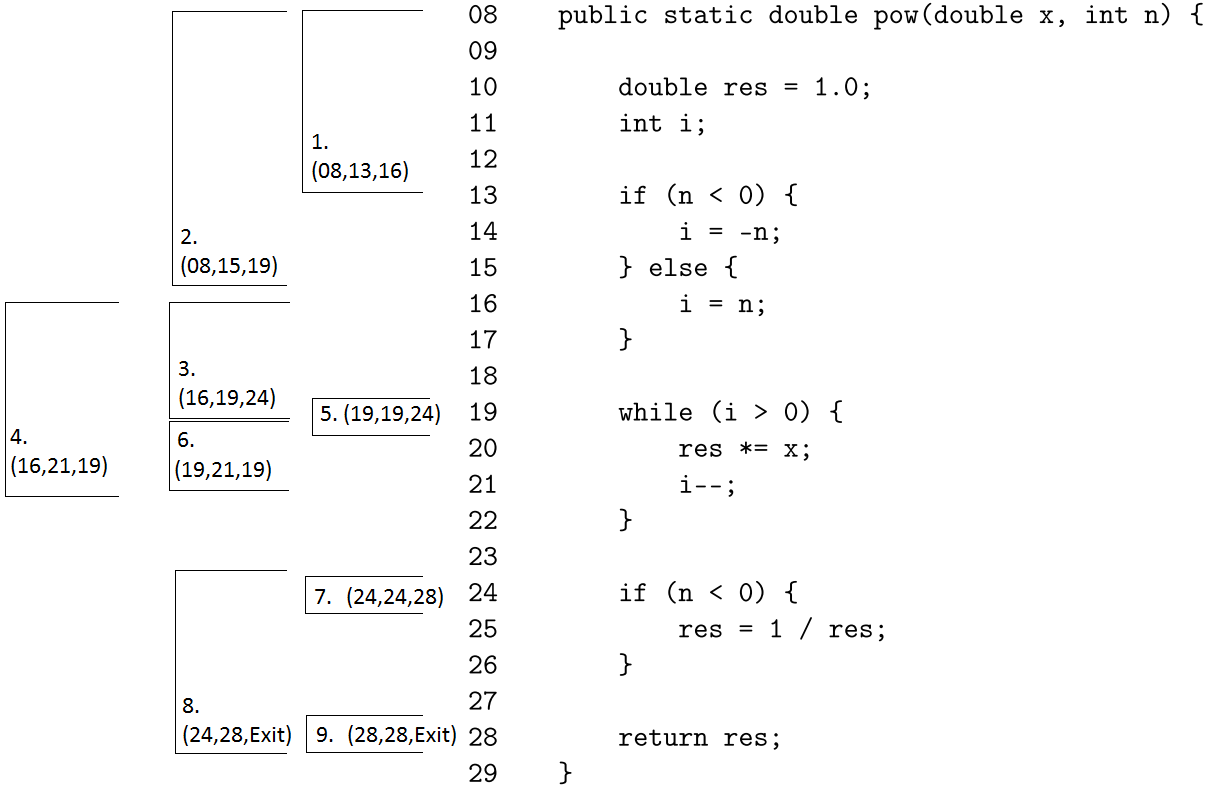
\includegraphics[width=\columnwidth]{Aufg6_1.png}
	%\end{figure}
  

  \section*{Aufgabe 6.2}

  \subsection*{(a) Kontrollflussgraph}
		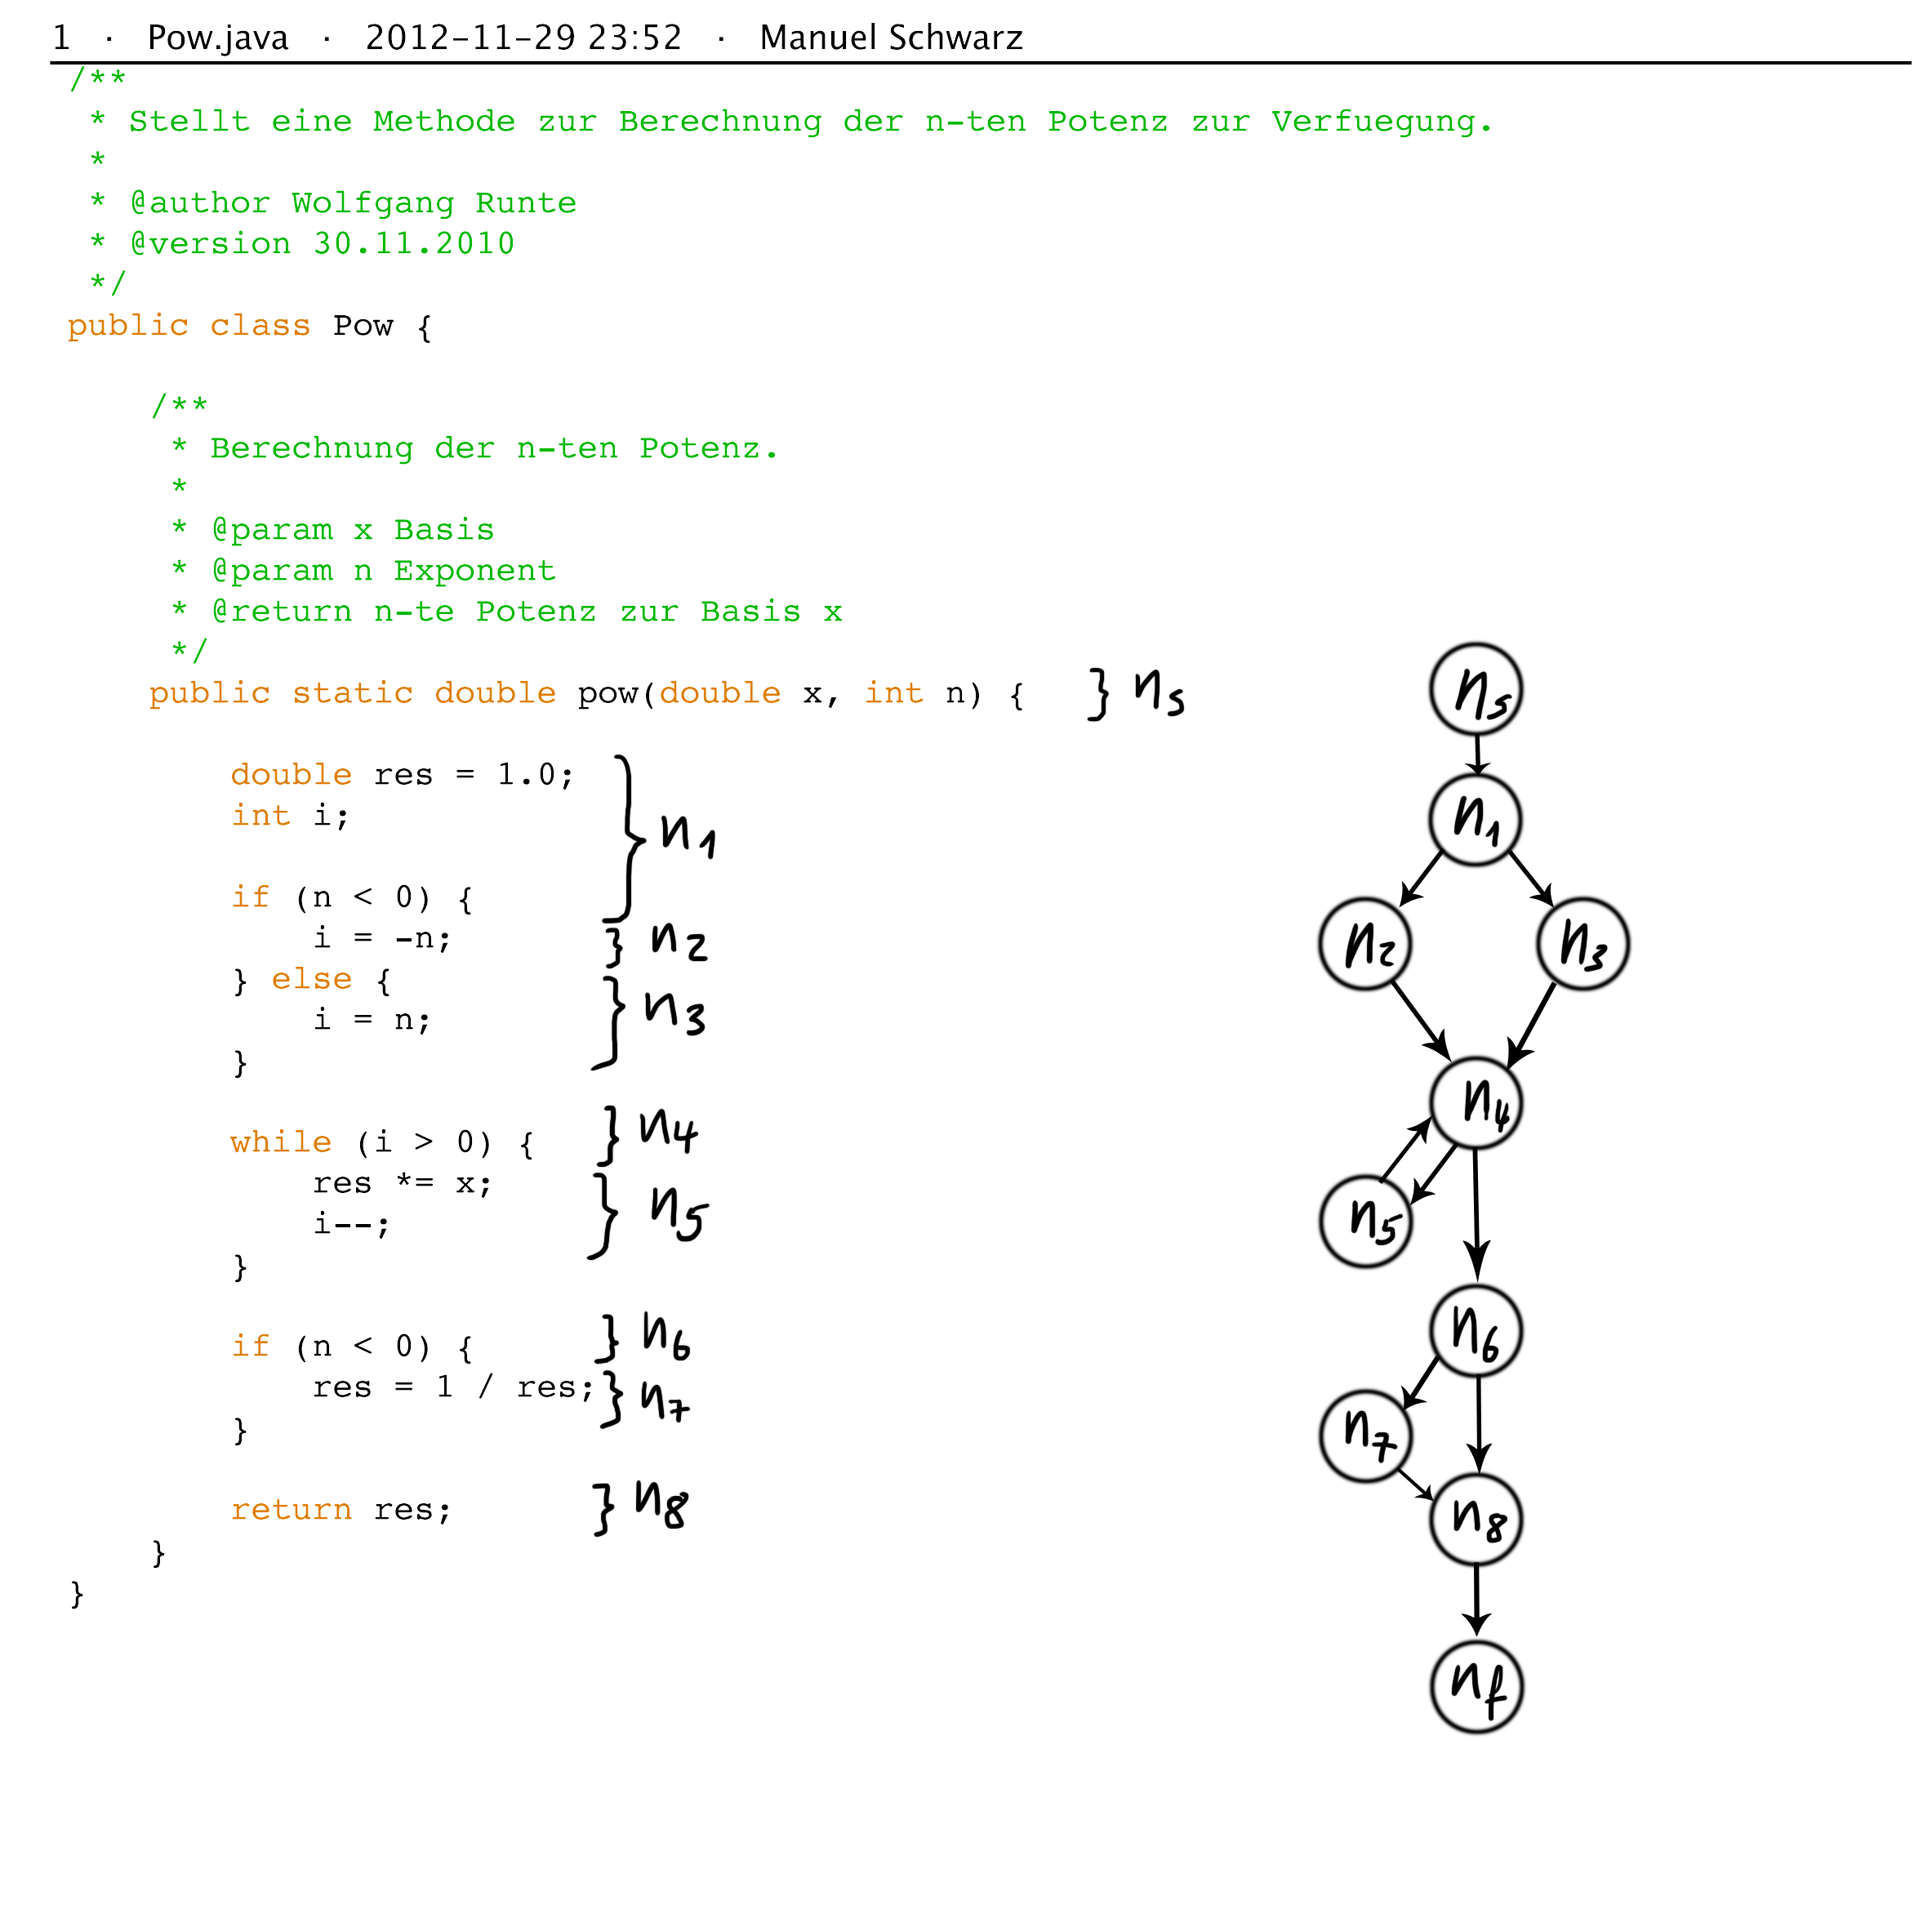
\includegraphics[width=\columnwidth]{Pow.png}

  \subsection*{(b) zyklomatische Komplexit�t}
  Die allgemeine Formel f�r die zyklomatische Komplexit�t eines Graphen $G$ lautet
  \begin{equation}
      Z(G) = e - n + 2
  \end{equation}
  Dabei beschreibt $e$ die Anzahl der Kanten und $n$ die Anzahl der Knoten von $G$.
  In unserem Fall gilt folglich:
  \begin{align*}
    Z(G) &= 12 - 10 + 2\\
    Z(G) &= 4
  \end{align*}


  \subsection*{(c)}

\end{document}
